\subsubsection{Fase 1}
\mbox{\hspace{-6ex}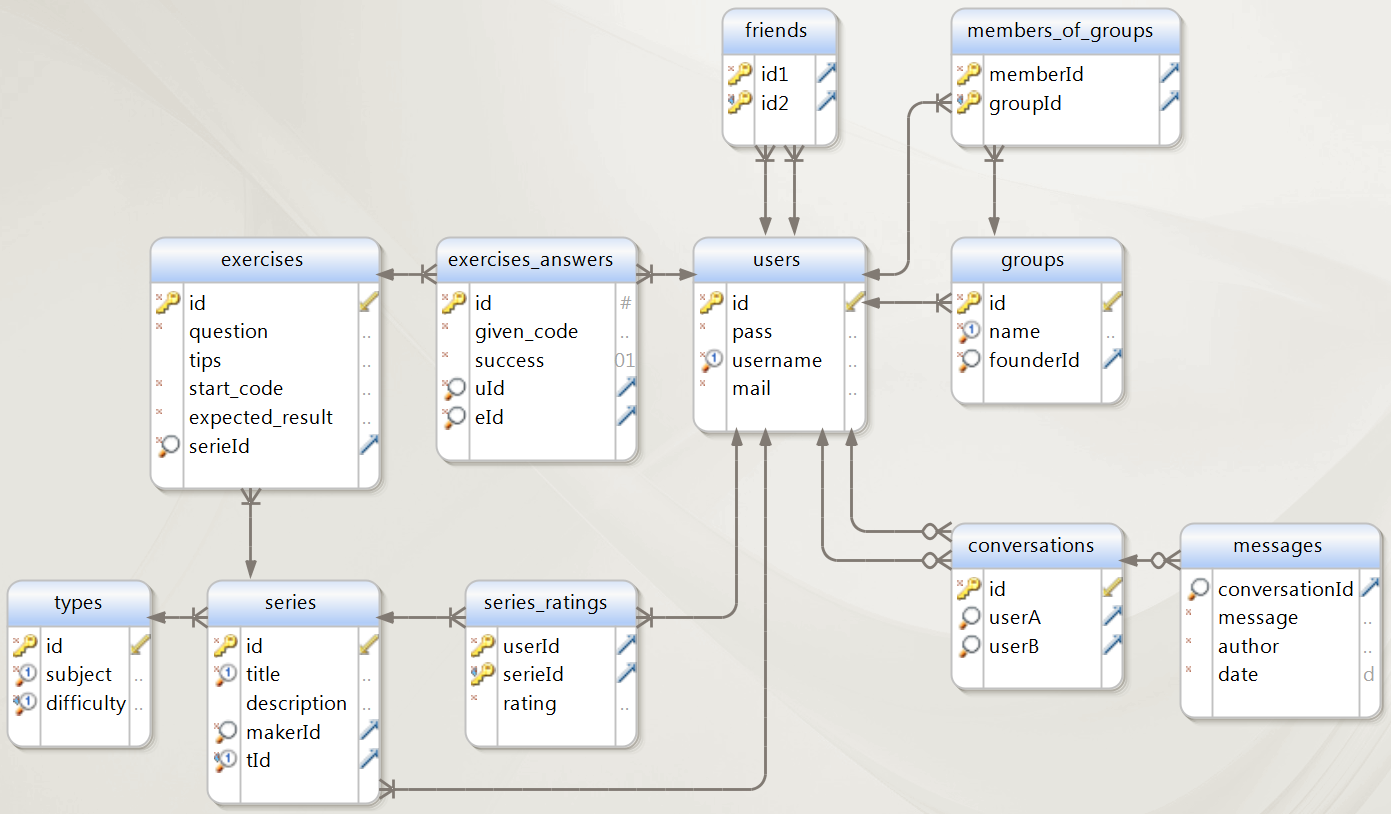
\includegraphics[keepaspectratio=true, scale=0.4]{raport_files/design/UML1.png}}
\subsubsection{Fase 2}
\mbox{\hspace{-6ex}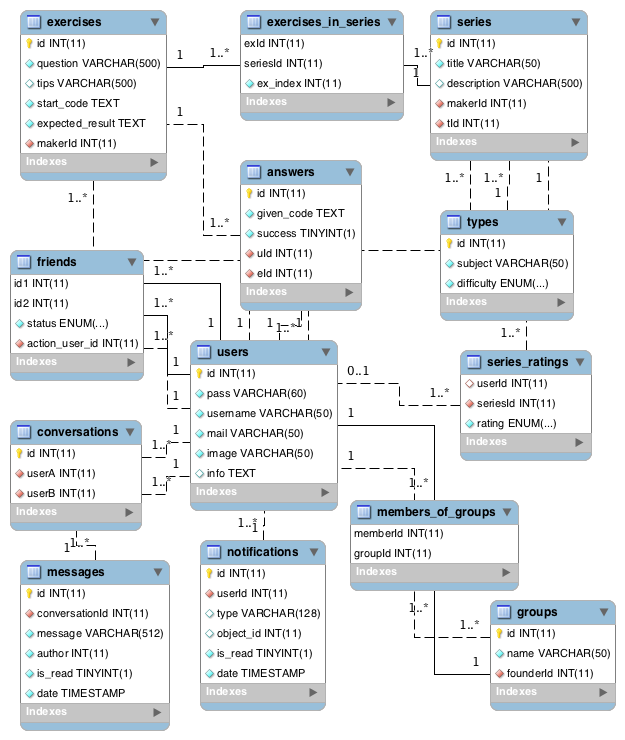
\includegraphics[keepaspectratio=true, scale=0.6]{raport_files/design/UML2.png}}\\
\subsubsection{Fase 3}
\mbox{\hspace{-6ex}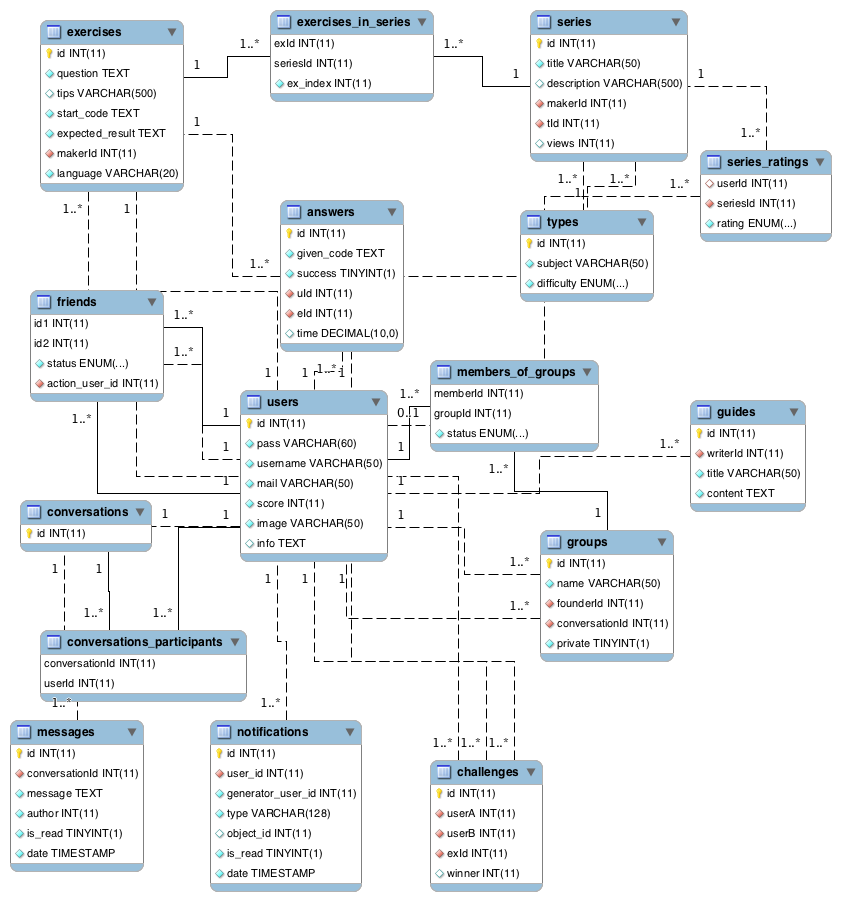
\includegraphics[keepaspectratio=true, scale=0.5]{raport_files/design/UML3.png}}\\
\small Hieronder wordt een korte uitleg gegeven over bovenstaande entiteiten. De uitbreiding van fase 2 t.o.v. fase 1
worden \textsl{licht cursief} weergegeven. De uitbreiding voor fase 3 in \textbf{vetgedrukt}.
\normalsize
\begin{description}
    \item[Users] zijn de essentie van de website. Zij maken uit hoe succesvol de website kan zijn.
        Een User is 'een geregistreerde bezoeker'. \textsl{Users zijn uitgebreid om nu een afbeelding
        te bevatten, alsook een (optionele) uitleg over de gebruiker.} \textbf{Users hebben nu een score,
        deze is de som van punten die je krijgt door "challenges" te winnen}.
    \item[Friends] is een 1-to-1 relatie. \textsl{Status kan waarden "pending", "accepted" en "declined" aannemen.
        action\_user\_id wordt gebruikt om na te kijken welke gebruiker als laatste de status heeft gepdatet.}
    \item[Conversations] \st{staat letterlijk voor een conversatie tussen 2 personen.} \textbf{bevat slechts een id
        om een conversatie voor te stellen.}
    \item[Conversations\_participants] \textbf{zijn gebruikers die deelnemen aan bepaalde conversaties.}
    \item[Messages] zijn de berichten die van een gebruiker in een conversatie gestuurd worden.
        \textsl{Gebruikers kunnen zien of hun bericht gelezen is of niet.} \\
        From/to attributen zijn gesplitst van Messsages om redundantie te vermijden.
    \item[Groups] zijn verzamelingen van Users. Een groep wordt opgericht door een gebuiker, de 'founder'
        van de groep. Meerdere Users kunnen dan zonder meer lid worden van de groep. De gebruikers kunnen
        nadien de groep verlaten (met uitzondering van de 'founder'). Dit maakt dat een groep altijd minstens
        1 lid heeft.
        \\\textbf{Groepen kunnen nu priv\'e of publiek zijn, en gebruiken conversations zodat de
        leden op de groepspagina kunnen chatten met elkaar.}
    \item[Members of groups] zijn de gebruikers die lid zijn van een groep. \textbf{Status kan waarden "pending",
        "accepted" en "declined" aannemen.}
    \item[Series] zijn het tweede essentiele deel van de applicatie. Een serie bestaat uit een set
        van 'Exercises'. Iedere serie krijgt ook een type en een rating.
        \textbf{d.m.v. views kunnen gebruikers zien hoe veel een oefeningenreeks al bekeken is.}
    \item[Series rating] zijn de ratings die gebruikers aan een serie kunnen geven. Deze rating
        zal gebruikt worden om voorstellen te doen aan andere gebruikers.
    \item[Types] zijn tuples van een onderwerp en een moeilijkheidsgraad. Deze tuple vormt een
        unieke key van het type.
    \item[Exercises] vormen samen een serie. Iedere exercise bevat een vraag, (optionele) tips voor
        het oplossen van de oefening, start code die de gebruiker een beginpunt geeft en een verwacht resultaat.
        Dit verwacht resultaat wordt vergeleken met de gegenereerde output van de interpreter. \textsl{Exercises
        zijn niet langer verbonden aan een enkele serie. Om dit mogelijk te maken is een extra relatie toegevoegd:
        exercises\_in\_series. Een bijkomende uitbreiding is de mogelijkheid om als verwacht antwoord een reguliere
        expressie te geven. Deze wordt dan gematched met de gegenereerde oplossing.}
        \textbf{language duidt aan of de oefening in python of c++ is.}
    \item[\textsl{Exercises\_in\_series}] \textsl{is een relatie tussen oefeningen en series. Hierin wordt gespecifieerd welke oefening
        in welke serie staat. Als bijkomend attribuut wordt de index van de oefening binnen de serie gespecifieerd.
        Hierdoor wordt de volgorde van oefeningen gecontroleerd. De beperking is opgesteld dat iedere oefening slechts 1x
        in een serie mag staan.}
    \item[Answers] zijn niet meer dan de aangepaste start code, samen met het resultaat
        van de interpreter. Zo kan een gebruiker de code later opnieuw opvragen en kan tegelijk snel
        opgevraagd worden of een gebruiker de oefening correct had opgelost.
        \textbf{time duidt aan hoe lang een gebruiker aan een oefening heeft gewerkt, dit wordt gebruikt
        bij "challenges".}
    \item[\textsl{Notifications}] \textsl{zijn meldingen die een gebruiker kan krijgen. Denk hierbij aan bijvoorbeeld een
        ontvangen vriendschapsverzoek. type is een korte beschrijving van de soort melding, object\_id(optioneel) is
        de id van een object relevant aan de melding.}
    \item[Challenges] \textbf{stellen een wedstrijd tussen 2 gebruikers voor om een oefening zo snel mogelijk af te maken.}
    \item[Guides] \textbf{kunnen gebruikt worden om gebruikers meer uitleg te geven om vanalles bij te leren. Guides kunnen bv
        een inleiding geven tot een bepaald concept en dan naar een oefeningenreeks linken.}
\end{description}
